\documentclass{beamer}
%
% Choose how your presentation looks.
%
% For more themes, color themes and font themes, see:
% http://deic.uab.es/~iblanes/beamer_gallery/index_by_theme.html
%
\mode<presentation>
{
  \usetheme{default}      % or try Darmstadt, Madrid, Warsaw, ...
  \usecolortheme{default} % or try albatross, beaver, crane, ...
  \usefonttheme{default}  % or try serif, structurebold, ...
  \setbeamertemplate{navigation symbols}{}
  \setbeamertemplate{caption}[numbered]
} 

\usepackage[english]{babel}
\usepackage[export]{adjustbox}
 % \usepackage[utf8x]{inputenc}
\usepackage[style=authoryear]{biblatex}
\addbibresource{references.bib}
\usepackage{tikz}
\graphicspath{{figures/}}
\DeclareMathOperator{\sign}{sign}

\usepackage{caption}
\captionsetup{font=scriptsize, labelfont=scriptsize}

\newcommand{\specialcell}[2][c]{%
  \begin{tabular}[#1]{@{}c@{}}#2\end{tabular}}

\title[Your Short Title]{When does vapor pressure deficit drive or reduce evapotranspiration?}
\author{Adam Massmann,  Pierre Gentine and Changjie Lin}
\institute{AGU Fall Meeting (Rough Draft)}
\date{December 14th, 2017}

\begin{document}

\begin{frame}
  \titlepage
\end{frame}


\section{Introduction}
\begin{frame}{Does VPD drive or reduce ET? - hydrometeorologists' perspective}
  \begin{Huge}
  \[VPD = (1-RH)\cdot e_s (T)\]
\end{Huge}
  \begin{itemize}
  \item \textbf{Hydrometeorologists} would say that an increase in VPD (increase in \textbf{atmospheric demand}) would drive an \textbf{increase in ET}.
  \end{itemize}
\end{frame}

\begin{frame}{Does VPD drive or reduce ET? - physiologists' perspective}
  \begin{figure}
  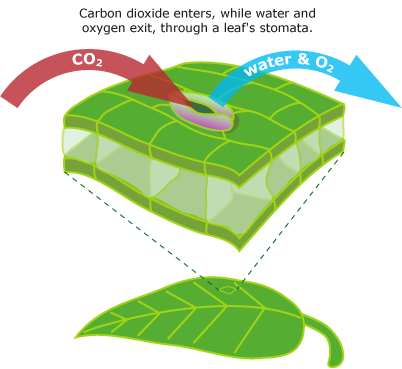
\includegraphics[width=2.25in]{stomata.png}% was O(1.5in)
  \caption{from evolution.berkeley.edu}
\end{figure}
  \begin{itemize}
  \item However, \textbf{plant physiologists} know that plants have evolved to use stomata to conserve and regulate water use. So \textbf{stomata closure} in response to increases in VPD may \textbf{decrease ET}.
  \end{itemize}
\end{frame}


\begin{frame}{The question is, which effect dominates with an increase in VPD: plant response (decrease in ET) or atmospheric demand (increase in ET)?}
  \begin{itemize}
  \item It should be a function of plant type and the environment:
    \begin{itemize}
    \item Plants that are evolved to conserve water will tend to reduce ET with increases in VPD.
    \item However the environment can overwhelm plant response: at some threshold (i.e. very high VPD) the atmospheric demand should dominate and plants will not be able to conserve water, no matter how much they have evolved to do so.
    \end{itemize}
  \end{itemize}
\end{frame}

\section{Method}
\begin{frame}{Use physically reasonable assumptions to develop a theory.}
  We can use Penman-Monteith (PM) to estimate ET:
  \[ET = \frac{\Delta R + g_a \rho_a c_p \, VPD}{\Delta + \gamma(1 + \frac{g_a}{g_s})},\]
\textbf{Problem}: $g_s$ (stomatal conductance) is a function of photosynthesis, which is a function of ET itself.  So ET in PM is really an implicit function of itself and we cannot take derivatives!
\end{frame}

\begin{frame}{Use physically reasonable assumptions to develop a theory.}
Apply a constant uWUE assumption (conserved within plant type; see \cite{Zhou_2016}):
\[uWUE = \frac{GPP \cdot \sqrt{VPD}}{ET},\]
To derive a new form of Penman-Monteith without implicit ET dependence:
  \[  ET = \frac{\Delta R + \frac{g_a\; P}{T} \left( \frac{ c_p \, VPD}{R_{air}} -  \frac{\gamma c_s \sqrt{VPD} }{ R* \; 1.6 \text{ uWUE } (1 + \frac{g_1}{\sqrt{VPD}})} \right)\footnote{note that all terms are known }}{ \Delta + \gamma}\]
\end{frame}

\begin{frame}{Use physically reasonable assumptions to develop a theory.}
  With our new form of Penman-Monteith we can now take derivatives, giving:
  \[\frac{\partial \;  ET}{\partial \, VPD} = \frac{2 g_a \; P}{T(\Delta + \gamma)}   \left(\frac{ c_p}{R_{air}} - \frac{\gamma c_s }{1.6 \; R*\; \text{ uWUE }} \left( \frac{2 g_1 + \sqrt{VPD}}{2 (g_1 + \sqrt{VPD})^2}\right) \right)\]
  In the interest of time, we will just focus in the ``sign'' term:
  \[\sign \left[\frac{\partial \;  ET}{\partial \, VPD}\right] = \sign \left[  \left(\frac{ c_p}{R_{air}} - \frac{\gamma c_s }{1.6 \; R*\; \text{ uWUE }} \left( \frac{2 g_1 + \sqrt{VPD}}{2 (g_1 + \sqrt{VPD})^2}\right) \right) \right] \]

\end{frame}

\section{Results - theory}
\begin{frame}{Consequences of theory - ``sign'' term}
  \[\frac{\partial \, ET}{\partial \, VPD} = \text{scaling} \cdot \left(\frac{ c_p}{R_{air}} - \frac{\gamma c_s }{1.6 \; R*\; \text{ uWUE }} \left( \frac{2 g_1 + \sqrt{VPD}}{2 (g_1 + \sqrt{VPD})^2}\right) \right)\]
  \begin{itemize}
  \item $c_p$ and $R*$ are constants
  \item $R_{air}$, $\gamma$, and $c_s$ are approximately constant (relative to $\sqrt{VPD}$)
  \item uWUE and $g_1$ are constants within plant type (i.e. grass, crops, deciduous forest, evergreen needleleaf forest, shrub)
  \item Which just leaves VPD
  \end{itemize}
  So within each plant type, whether the atmospheric demand (ET increasing with VPD) or plant response (ET decreasing with VPD) dominates is essentially just a function of VPD!
\end{frame}

\begin{frame}{``Sign'' Term}
  \begin{figure}
    \adjincludegraphics[width=3.5in, trim={0 {0.51\height} 0 0}, clip]{fig05.pdf}
  \end{figure}
\end{frame}


\section{Test Theory}
\begin{frame}{The theory seems nice, but we should test with data!}
    \begin{itemize}
    \item Introduce a free uncertainty parameter $\sigma$ to Penman Monteith:
      \[ET = \frac{\Delta R + \frac{g_a\; P}{T} \left( \frac{ c_p VPD}{R_{air}} -  \frac{\gamma c_s \sqrt{VPD} }{ R* \; 1.6\; \boldsymbol{\sigma} \; \text{ uWUE } (1 + \frac{g_1}{\sqrt{VPD}})} \right) }{ \Delta + \gamma}\]
    \item At each observation from FLUXNET (56 sites across globe) calculate a unique $\sigma$:
      \small
      \[\sigma = - \frac{g_a \gamma c_s \sqrt{VPD} P }{ \left(\text{ ET } ( \Delta + \gamma) - \Delta R - g_a \rho_a c_p VPD\right) 1.6 \; R\; T\; \text{ uWUE } (1 + \frac{g_1}{\sqrt{VPD}})}\]
      \normalsize
    \item Then propagate uncertainty forward by including $\sigma$ in the derivative:
    \end{itemize}
      \[\frac{\partial \;  ET}{\partial \; VPD} = \text{scaling} \cdot \left(\frac{ c_p}{R_{air}} -  \frac{\gamma c_s }{1.6 \; R*\; \sigma \; \text{ uWUE }} \left( \frac{2 g_1 + \sqrt{VPD}}{2 (g_1 + \sqrt{VPD})^2}\right) \right)\]

  \end{frame}
  
    \begin{frame}{Test theory with FLUXNET data - CSH}
                \includegraphics[width=3.5in]{csh_eee.png}
     \end{frame}


    \begin{frame}{Test theory with FLUXNET data - ENF}
                \includegraphics[width=3.5in]{enf_eee.png}
     \end{frame}


    \begin{frame}{Test theory with FLUXNET data - DBF}
                \includegraphics[width=3.5in]{dbf_eee.png}
     \end{frame}

    \begin{frame}{Test theory with FLUXNET data - CRO}
                \includegraphics[width=3.5in]{cro_eee.png}
     \end{frame}

    \begin{frame}{Test theory with FLUXNET data - GRA}
                \includegraphics[width=3.5in]{gra_eee.png}
     \end{frame}



% \begin{frame}{Summary of theory}
%   \begin{itemize}
%   \item We use \cite{Zhou_2016}'s uWUE to derive a new analytically tractable form of PM.
%   \item This new analysis suggests that the ``tipping'' point for which atmospheric demand overwhelms plant response will be almost exclusively a function of VPD.
%     \begin{itemize}
%     \item For each PFT there will be a VPD$_{crit}$ above which atmospheric demand will dominate and ET will increase with VPD.
%     \end{itemize}
%   \item Plant types evolved to conserve water (CSH) have a higher VPD$_{crit}$ than plants evolved (or bred) to use water and prioritize GPP (CRO). Trees and grasslands are somewhere between these two extremes.
%   \item Aerodynamic conductance scales the response, so plants with large surface roughness will be more likely to have a larger response as there is less resistance between the surface and the atmosphere.
%   \end{itemize}
% \end{frame}


\section{Conclusions}
% \begin{frame}{Summary}
%   \begin{itemize}
%   \item Theory finds that the ``tipping'' point for which atmospheric demand overwhelms plant response will be almost exclusively a function of VPD.  Plant types evolved to conserve water (CSH) have a higher VPD$_{crit}$ (and more negative ET response) than plants evolved (or bred) to use water and prioritize GPP (CRO).
%   \item On average, ecosystem response to VPD follows roughly what we might expect: CRO (prioritize GPP) has positive ET response to VPD, while all others have a negative response. Ordering by increasing magnitude of negative response gives: DBF, GRA, ENF, CSH; which roughly correspond to expectations for increasing water conservation as a function of PFT.
%   \item Uncertainty is high, especially for CRO and GRA. However, inclusion of uncertainty does not change the story for ENF or CSH.
%   \end{itemize}
% \end{frame}


\begin{frame}{Summary}
  \small
  \begin{itemize}
  \item Derived a new form of Penman-Monteith that explicitly calculates ET given published constants.
  \item Developed a theory for when atmospheric dryness will increase ET (atmospheric demand dominates) vs. decrease ET (plant response dominates). Theory tests well using real data from FLUXNET2015 on plant types CSH, ENF, and DBF. Applicability to CRO and GRA is more uncertain.
  \item For plants evolved to prioritize water conservation over production, atmospheric demand is less likely to dominate.
  \item All plant types except for crops had common occurrence of decreases in ET with increases in VPD (plant response dominates). Therefore, the hydrometeorologists perspective is often wrong, and drought indices built upon assumptions about atmospheric demand are unrealistic for vegetated surfaces.
  \item Our form of Penman-Monteith is capable of estimating ET realistically and could be used as a replacement for PET in drought indices (e.g. Palmer Drought Severity Index - PDSI).
  \end{itemize}
\end{frame}

\section{References}
\begin{frame}{References}
  \AtNextBibliography{\small}
  \printbibliography
  \scriptsize
  \begin{itemize}
  \item This work used eddy covariance data acquired and shared by the FLUXNET community, including these networks: AmeriFlux, AfriFlux, AsiaFlux, CarboAfrica, CarboEuropeIP, CarboItaly, CarboMont, ChinaFlux, Fluxnet-Canada, GreenGrass, ICOS, KoFlux, LBA, NECC, OzFlux-TERN, TCOS-Siberia, and USCCC. The ERA-Interim reanalysis data are provided by ECMWF and processed by LSCE. The FLUXNET eddy covariance data processing and harmonization was carried out by the European Fluxes Database Cluster, AmeriFlux Management Project, and Fluxdata project of FLUXNET, with the support of CDIAC and ICOS Ecosystem Thematic Center, and the OzFlux, ChinaFlux and AsiaFlux offices.
    \item This material is based upon work supported by the National Science Foundation Graduate Research Fellowship under Grant No. DGE 16-44869. Any opinion, findings, and conclusions or recommendations expressed in this material are those of the authors(s) and do not necessarily reflect the views of the National Science Foundation.
    \end{itemize}
\end{frame}

\section{Extra Slides}

\begin{frame}{Extra slide - statistics}
  \begin{table}
  \label{vpd_crit}
\caption{More quantitative test of theory.}
\centering
\begin{tabular}{l c c c c c c}
  \hline
  PFT & \specialcell{Fraction of Obs.\\Theory is Correct} & Mean ($\frac{\partial \; ET}{\partial \; VPD} < 0$) & Mean ($\frac{\partial \; ET}{\partial \; VPD} > 0$)\\
  \hline
  CRO & 0.566517 & -0.209152 &  0.005856\\
  CSH & 0.931660 & -0.264746 &       NaN\\
  DBF & 0.633363 & -0.135679 &  0.042910\\
  ENF & 0.633138 & -0.150665 &  0.029281\\
  GRA & 0.442306 & -0.042158 & -0.042480\\
  \hline
\end{tabular}
\end{table}
\end{frame}

\begin{frame}{Extra slide - is theory VPD$_{crit}$ optimum?}
  \includegraphics[width=\textwidth]{for_agu.pdf}
\end{frame}

% \begin{frame}{Summary statistics - extra sl}
%      \begin{table}
%        \caption{Statistics of $\frac{\partial \; ET}{\partial \, VPD}$ as a function of PFT.}
%        \centering
%        \begin{tabular}{l c c}
%          \hline
%          PFT & $\overline{\frac{\partial \; ET}{\partial \; VPD}}$ & fraction $\frac{\partial \; ET}{\partial \; VPD} < 0.$ \\
%          \hline
%          CRO & 0.000853  & 0.473311\\
%          CSH & -0.108234 & 0.931660\\
%          DBF & -0.012727 & 0.461674\\
%          ENF & -0.034087 & 0.534425\\
%          GRA & -0.019637 & 0.631735\\
%          \hline
%          \multicolumn{2}{l}{}  
%        \end{tabular}
%      \end{table}
%    \end{frame}
     




% \begin{table}
% \centering
% \begin{tabular}{l|r}
% Item & Quantity \\\hline
% Widgets & 42 \\
% Gadgets & 13
% \end{tabular}
% \caption{\label{tab:widgets}An example table.}
% \end{table}

\end{document}
